\chapter{Élaboration  et évaluation du modèle de prédiction }
Tous au long de ce chapitre nous allons entrainer nos algorithmes de prédiction avec des données provenant de chaque faculté et essayerons de prédire le CGPA, nous  avons utiliser des algorithmes présentés au chapitre premier pour entrainer nos modèles de prédiction.
Pour choisir l'algorithme à utiliser nous sommes basés sur la documentation officielle de la librairie scikit-learn \cite{pedregosa2011scikit} qui nous a fourni l'infographie sur la figure \ref{fig:skLearn1} pour le choix des algorithmes. \\

\begin{figure}[ht]
	\centering
	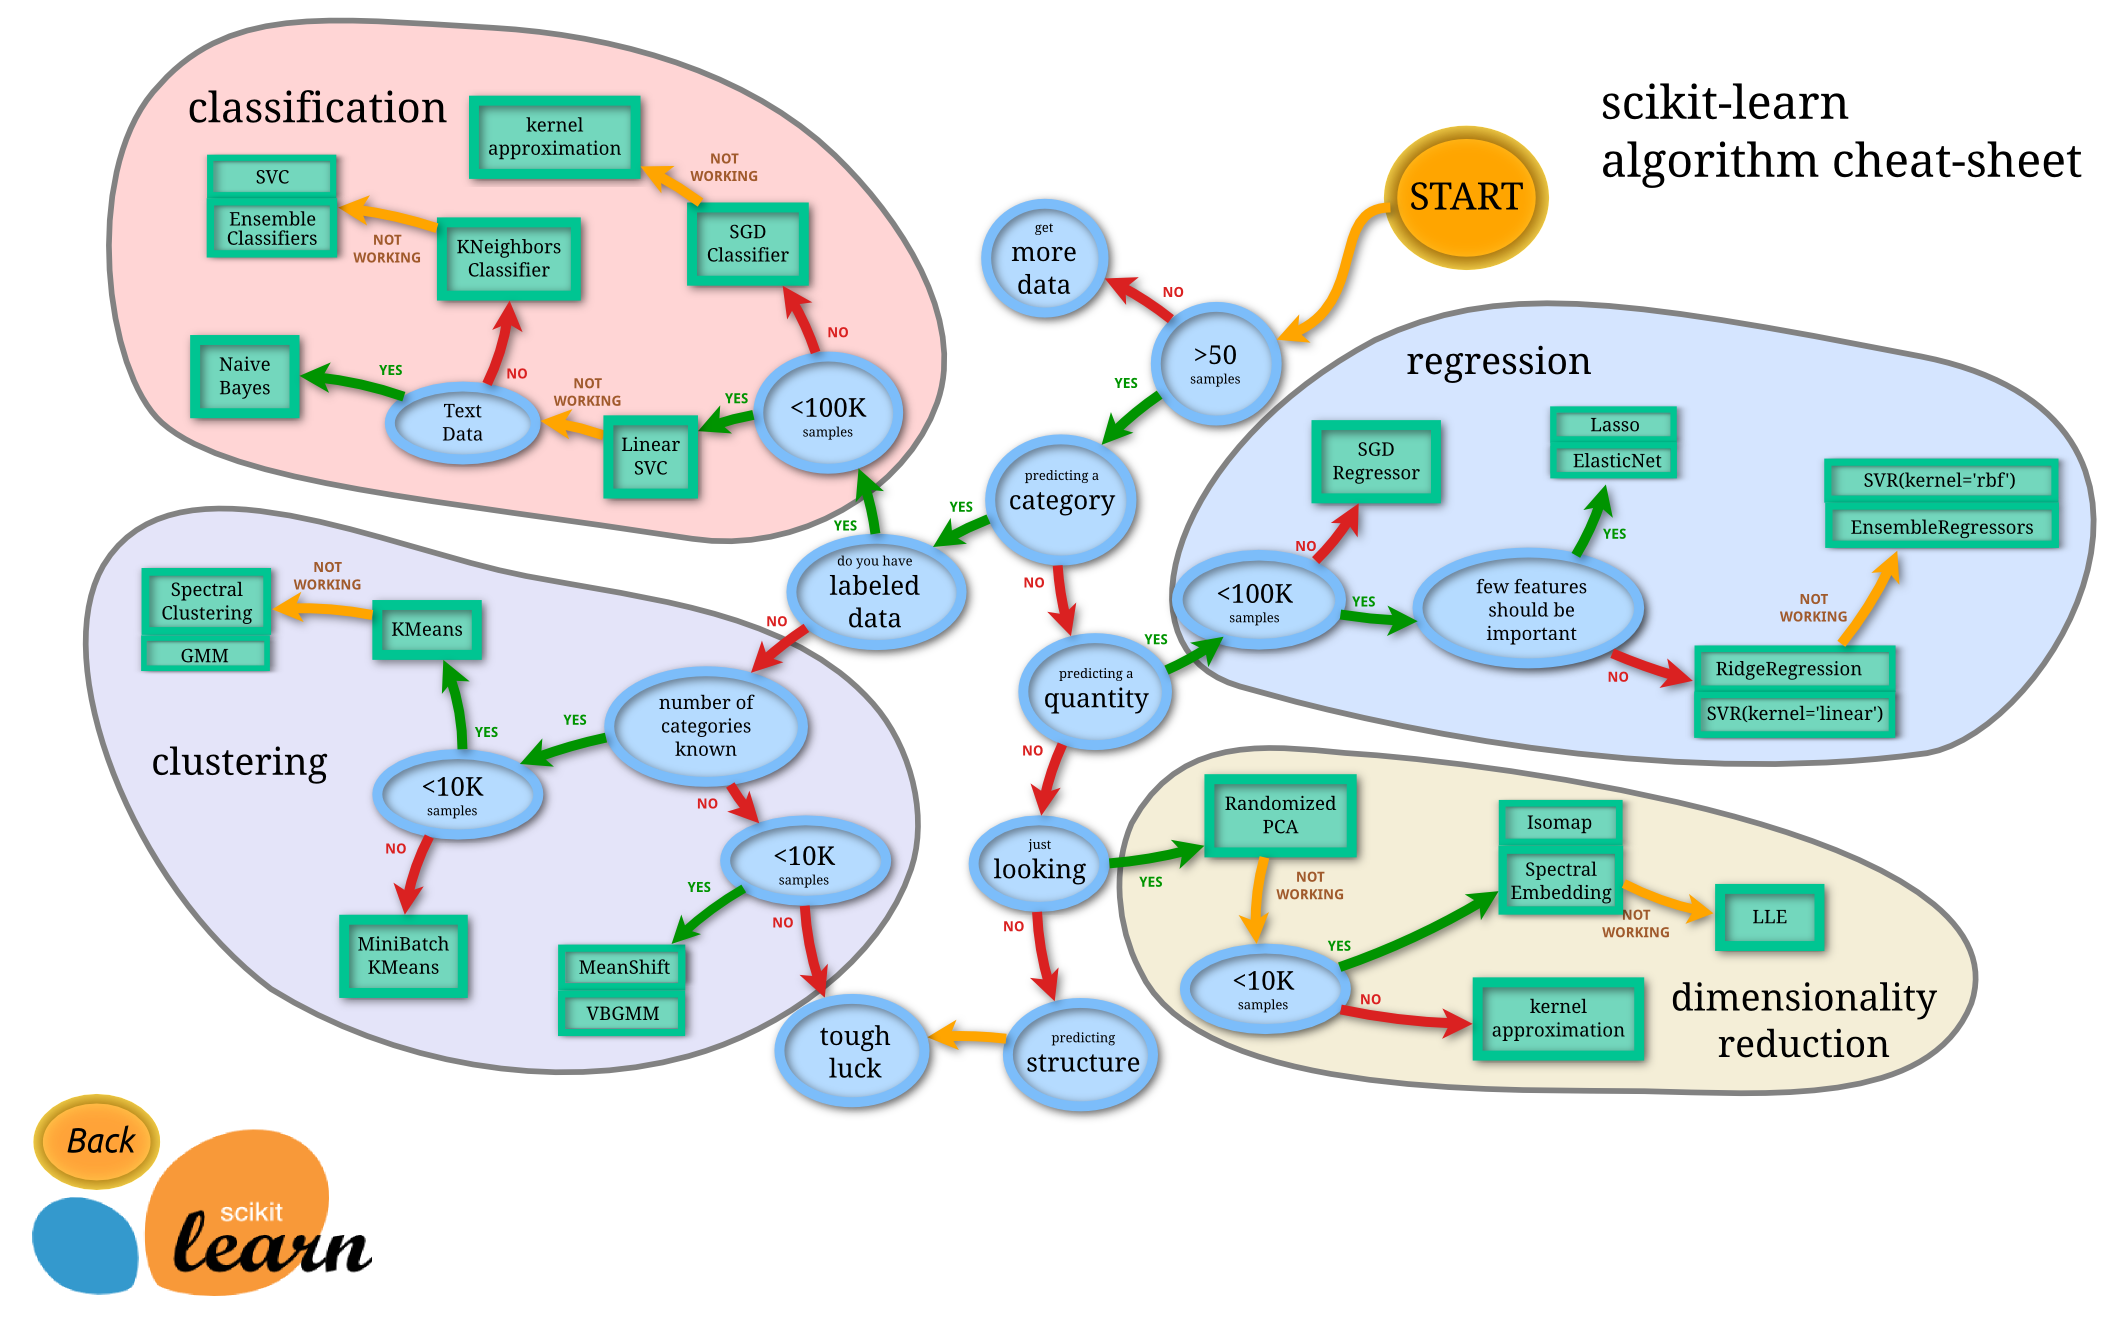
\includegraphics[width=0.5\textwidth]{fig/sckikLearnCheatSheet.png}
	\caption{sckit-Learn Algorithm cheat sheet }
	\label{fig:skLearn1}
\end{figure}  

Vu que nous disposons de moins de 100000 instances pour nos ensemble d'apprentissage et vu que notre tache était celui de prédire une variable continue (Une régression )  nous avons décidé d'entrainer les algorithmes  suivantes :
\begin{enumerate}
	\item Ridge Régression
	\item Elastic Net Régression
	\item Lasso Régression
	\item \ac{SVR} avec Kernel Linéaire
	\item  \ac{SVR} avec Kernel Gaussien 
\end{enumerate}
Les 3 premiers modèles sont des versions issues de la régularisation de la régression linéaire vu au chapitre 1  et qui conviennent bien pour des ensembles d'apprentissages relativement petits , le 2 derniers sont une adaptation du \ac{SVM} pour la régression.\\
Notons que toutes ses librairies sont bien implémentées et optimisées dans scikit-learn.
Tous au long de ce chapitre nous avons suivie les étapes suivantes  sur la figure \ref{fig:predictiveModelBuilding}:
 \begin{enumerate}
 \item Préparation des données :
 \begin{itemize}
 	\item  Encodage One Hot
 	\item  Normalisation
 	\item  Échantillonnage
 \end{itemize}
\item Exécution des algorithmes
\item évaluation 
   \begin{itemize}
  	\item  Évaluation sur l'ensemble d'apprentissage (training set)
  	\item  Validation croisée sur l'ensemble d'apprentissage
  	\item  Évaluation sur l'ensemble d'évaluation (test set) 
  \end{itemize}
\item Amélioration des modèles par les méthodes d'ensembles
\item Évaluation du modèle finale
 \end{enumerate}
\begin{figure}[ht]
	\centering
	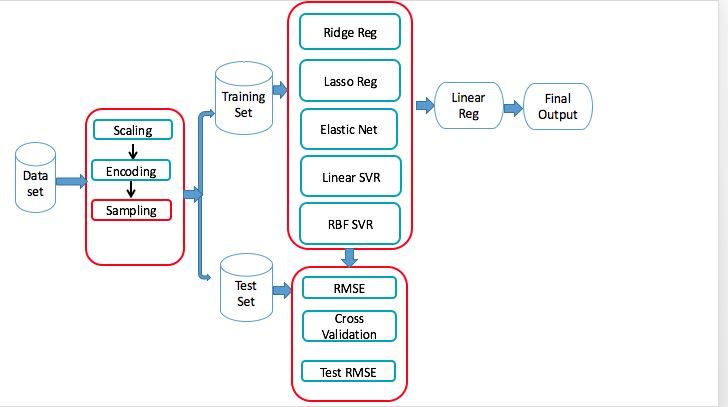
\includegraphics[width=0.5\textwidth]{fig/ModelBuilding.png}
	\caption{étapes à suivre pour l'élaboration du modèle d'apprentissage }
	\label{fig:predictiveModelBuilding}
\end{figure} 
\section {Préparation des données pour l'exécution des algorithmes } 
Dans cette partie nous expliquerons comment s'est passé la préparation des nos données , rappelons que notre ensemble d'apprentissage finale dispose de 4 attributs et notre valeur à prédire :
\begin{enumerate}
	\item  SCHOOLNAME : de nature catégorielle (string)
	\item  OPTION : de nature catégorielle (string)
	\item  DIPPERC : de nature continue (float)
	\item  CGPA : de nature continue (float)
\end{enumerate}
Comme l'a souligné \cite{OneHotEncoding} la librairie scikit learn ne travaille qu'avec les variables numériques , c'est pourquoi nous avons décider de transformer nos variables catégorielles les chaines de caractères en variables numériques en utilisant la technique du \emph{\textbf{One Hot encoding}} 
\subsection{Encodage des Variables One Hot }
Un encodage one-hot consiste à représenter des états en utilisant pour chacun une valeur dont la représentation binaire n'a qu'un seul chiffre 1.

On peut définir une fonction d'encodage one-hot comme étant la fonction qui prend en entrée un vecteur  z et qui redéfinit en sortie la plus grande valeur de  z à 1 et toutes autres valeurs de  z à 0.
L'avantage principal de cet encodage est que pour passer d'un état à un autre, seules deux transitions sont nécessaires : un chiffre passe de 1 à 0, un autre de 0 à 1. Son inconvénient est qu'il faut au minimum n bits pour représenter n états, ce qui conduit à une augmentation linéaire du nombre de chiffres par rapport au nombre d'états. Un encodage utilisant toutes les valeurs binaires existantes a quant à lui une augmentation logarithmique du nombre de chiffres.

Pour notre ensemble , après notre encodage nous pouvons aisément remarquer que notre ensemble d'apprentissage vient de passer de (4715, 4 )à (4715 , 647)  dimensions.
Mais ces dimension restent raisonnables pour un projet de machine Learning. 
\subsection{Normalisation  } 
Nous avons ensuite normalisé nos données pour les variables numériques en divisant le pourcentage du diplôme d'état par 100 et celui du CGPA,ceci pour permettre une exécution rapide de nos algorithmes. 
\subsection{Échantillonnage  \cite{statBook1} } 
Pour commencer notre entrainement nous avons échantillonné nos donnes pour constituer un ensemble d'apprentissage (Training set), et un ensemble d'évaluation du modèle (test set). Notre Training set était constituer de 80 \% de nos données et les 20 autres pour cent ont constitué notre ensemble d'évaluation.
Pour ce faire nous avons utilisé un échantillonnage stratifié.
Lorsqu'on utilise l'échantillonnage stratifié, on divise la population en groupes homogènes (appelés strates), qui sont mutuellement exclusifs, puis on sélectionne à partir de chaque strate des échantillons indépendants. On peut utiliser n'importe quelle des méthodes d'échantillonnage  pour sélectionner l'échantillon à l'intérieur de chaque strate. La méthode d'échantillonnage peut varier d'une strate à une autre. Lorsqu'on utilise l'échantillonnage aléatoire simple pour sélectionner l'échantillon à l'intérieur de chaque strate, on appelle le plan d'échantillonnage un plan d'échantillonnage aléatoire simple stratifié. On peut stratifier avant l'échantillonnage une population au moyen de toute variable dont on dispose pour la totalité des unités , pour notre étude nous avons utilisé la variable \textbf{EchecRatio}.

A la fin de cette phase nous avons pu obtenir un ensemble d'apprentissage (Training Set) et Un ensemble d'évaluation (Test Set )

\section {Élaboration et Évaluation du Modèle de Prédiction au sein de Chaque faculté} 
Dans cette section nous allons entrainer les différents algorithmes de prédictions avec les données de issue de chaque faculté et ensuite nous évaluerons le modèles sur les 2 ensembles.

Mais avant d'attaquer l'entrainement de nos modèle nous expliquerons nos métriques d'évaluations.
\subsection{Techniques D'évaluation} 
\subsubsection{\ac{RMSE} \cite{ProbaStat} }
C'est la racine carrée de la somme des carrées des différences entres les valeurs exactes et celles prédite par un modèle de prédiction pour chaque élément d'un ensemble d'apprentissage .
Il se donne par la formule suivante  :

 $RMSE=\sqrt{\frac{\sum _{=1}^{N}{\left[{h}_{\theta}\left({x}^{(i)}\right) - {y}^{(i)}\right]}^2} {N}}$
 
 Il constituera notre métrique d'évaluation pour tous nos modèles.
\subsubsection{Validation Croisé  \cite{CrossValidation}}
La validation croisée (« cross-validation ») est une méthode d’estimation de fiabilité d’un modèle fondé sur une technique d’échantillonnage. En fait, il y a au moins trois techniques de validation croisée : « test set validation » ou « holdout method », « k-fold cross-validation » et \ac{LOOCV} .
\begin{itemize}
	\item La première méthode est très simple, il suffit de diviser l'échantillon de taille n en deux sous échantillons, le premier d'apprentissage (communément supérieur à 60 \% de l'échantillon) et le second de test. Le modèle est bâti sur l'échantillon d'apprentissage et validé sur l'échantillon de test. L'erreur est estimée en calculant un test, une mesure ou un score de performance du modèle sur l'échantillon de test, par exemple l'erreur quadratique moyenne.
	\item Dans la seconde, on divise l'échantillon original en k échantillons, puis on sélectionne un des k échantillons comme ensemble de validation et les (k-1) autres échantillons constitueront l'ensemble d'apprentissage. On calcule comme dans la première méthode le score de performance. Puis on répète l'opération en sélectionnant un autre échantillon de validation parmi les (k-1) échantillons qui n'ont pas encore été utilisés pour la validation du modèle. L'opération se répète ainsi k fois pour qu'en fin de compte chaque sous-échantillon ait été utilisé exactement une fois comme ensemble de validation. La moyenne des k erreurs quadratiques moyennes est enfin calculée pour estimer l'erreur de prédiction. 
	\item La troisième méthode est un cas particulier de la deuxième méthode où k=n, c'est-à-dire que l'on apprend sur (n-1) observations puis on valide le modèle sur la énième observation et l'on répète cette opération n fois . 
\end{itemize}

Tous au long de ce chapitre nous avons utilisé les 2 premières techniques , nous n'avons pas utiliser la 3 ème technique car elle est trop gourmande  en termes des ressources(temps et mémoire) 

Nous pouvons maintenant attaquer l'entrainement des modèles au sein de chaque faculté  :
\subsection{Résultat des différents algorithmes par faculté}
Le tableau qui va suivre décrira les différentes algorithmes que nous avons entrainer pour les données de chaque faculté , chaque modèles dispose des paramètres ainsi que des différentes erreurs.
\begin{table} 
	\begingroup % make the next setting local
	\captionsetup{type=table} % here we want to caption a table
	\caption{Résultat des Algorithmes 1 ere iteration }
	\label{tab:AlgoResults}
	\noindent
	{\resizebox*{\textwidth}{\textheight}{%
			\renewcommand{\arraystretch}{2}
			\begin{tabular}{|c|c|c|c|c|c|c|c|}
				\toprule
				\multirow{6}{*}{} Faculté & Dimensions &Modèle &RMSE Train &\multicolumn{2}{c|}{CV Score}&RMSE Test &       STACK\_RES  \\
				\cline{5-6}
				&&&&M&std&& \\
				\cline{1-8}
				        &              &  ElasticNet &  0.06 : 11.14\% &  0.080  : 14.46\% &       0,0051 &  0.08 : 14.198\% &                  \\ \cline{3-8}
				&              &       Ridge &  0.07 : 11.83\% &  0.080  : 14.37\% &       0,0054 &  0.08 : 13.667\% &                  \\ \cline{3-8}
				FSTA &   (903, 240) &   LinearSVR &  0.06 : 11.51\% &  0.080  : 14.48\% &       0,0055 &  0.08 : 13.803\% &  0.062 : 11.132\% \\ \cline{3-8}
				&              &         SVR &  0.08 : 14.02\% &  0.080  : 14.44\% &       0,0058 &  0.08 : 13.667\% &                  \\ \cline{3-8}
				&              &       Lasso &  0.06 : 11.15\% &  0.082  : 14.85\% &       0,0072 &  0.08 : 14.151\% &                  \\ \cline{1-8}
				&              &  ElasticNet &   0.03 : 4.64\% &  0.079  : 12.70\% &       0,0223 &  0.08 : 12.247\% &                  \\ \cline{3-8}
				&              &       Ridge &   0.05 : 7.59\% &  0.088  : 14.13\% &       0,0122 &  0.10 : 15.534\% &                  \\ \cline{3-8}
				FT &   (140, 105) &   LinearSVR &   0.04 : 6.42\% &  0.085  : 13.69\% &       0,0129 &  0.09 : 14.646\% &   0.029 : 4.639\% \\ \cline{3-8}
				&              &         SVR &   0.06 : 9.88\% &  0.065  : 10.50\% &       0,0114 &  0.07 : 10.973\% &                  \\ \cline{3-8}
				&              &       Lasso &   0.03 : 4.65\% &  0.113  : 18.25\% &       0,0434 &  0.08 : 12.398\% &                  \\ \cline{1-8}
				&              &  ElasticNet &   0.05 : 8.43\% &  0.059  : 10.41\% &       0,0052 &  0.06 : 10.638\% &                  \\ \cline{3-8}
				&              &       Ridge &   0.05 : 9.19\% &  0.063  : 11.14\% &       0,0074 &  0.06 : 11.226\% &                  \\ \cline{3-8}
				FSEG &  (1549, 286) &   LinearSVR &   0.05 : 8.85\% &  0.063  : 11.15\% &       0,0082 &  0.06 : 11.270\% &   0.048 : 8.426\% \\ \cline{3-8}
				&              &         SVR &  0.06 : 10.92\% &  0.063  : 11.10\% &       0,0060 &  0.06 : 11.160\% &                  \\ \cline{3-8}
				&              &       Lasso &   0.05 : 8.46\% &  0.065  : 11.49\% &       0,0124 &  0.07 : 11.993\% &                  \\ \cline{1-8}
				&              &  ElasticNet &   0.05 : 8.01\% &  0.067  : 11.41\% &       0,0069 &  0.07 : 11.800\% &                  \\ \cline{3-8}
				&              &       Ridge &   0.06 : 9.34\% &  0.073  : 12.35\% &       0,0081 &  0.07 : 11.782\% &                  \\ \cline{3-8}
				FSDC &   (758, 257) &   LinearSVR &   0.05 : 8.87\% &  0.074  : 12.50\% &       0,0083 &  0.07 : 11.892\% &   0.047 : 8.007\% \\ \cline{3-8}
				&              &         SVR &  0.07 : 11.92\% &  0.072  : 12.22\% &       0,0037 &  0.07 : 12.353\% &                  \\ \cline{3-8}
				&              &       Lasso &   0.05 : 8.03\% &  0.081  : 13.78\% &       0,0206 &  0.07 : 11.711\% &                  \\ \cline{1-8}
				&              &  ElasticNet &   0.05 : 8.34\% &  0.070  : 12.04\% &       0,0068 &  0.08 : 13.020\% &                  \\ \cline{3-8}
				&              &       Ridge &   0.05 : 9.46\% &  0.074  : 12.73\% &       0,0092 &  0.07 : 12.882\% &                  \\ \cline{3-8}
				FD &   (896, 300) &   LinearSVR &   0.05 : 8.95\% &  0.074  : 12.78\% &       0,0097 &  0.08 : 13.022\% &   0.048 : 8.333\% \\ \cline{3-8}
				&              &         SVR &  0.07 : 11.54\% &  0.069  : 11.90\% &       0,0052 &  0.07 : 12.251\% &                  \\ \cline{3-8}
				&              &       Lasso &   0.05 : 8.36\% &  0.078  : 13.52\% &       0,0140 &  0.08 : 12.991\% &                  \\ \cline{1-8}
				&              &  ElasticNet &   0.04 : 7.80\% &  0.066  : 11.51\% &       0,0090 &  0.07 : 11.362\% &                  \\ \cline{3-8}
				&              &       Ridge &   0.05 : 8.78\% &  0.068  : 11.77\% &       0,0131 &  0.07 : 12.984\% &                  \\ \cline{3-8}
				FM &   (242, 111) &   LinearSVR &   0.05 : 8.28\% &  0.067  : 11.57\% &       0,0118 &  0.07 : 12.974\% &   0.045 : 7.798\% \\ \cline{3-8}
				&              &         SVR &  0.07 : 11.62\% &  0.070  : 12.05\% &       0,0120 &  0.07 : 12.493\% &                  \\ \cline{3-8}
				&              &       Lasso &   0.04 : 7.80\% &  0.068  : 11.73\% &       0,0098 &  0.08 : 14.448\% &                  \\ \cline{1-8}
				&              &  ElasticNet &   0.04 : 7.49\% &  0.081  : 13.62\% &       0,0082 &  0.06 : 10.747\% &                  \\ \cline{3-8}
				&              &       Ridge &   0.06 : 9.49\% &  0.089  : 14.90\% &       0,0159 &  0.07 : 11.120\% &                  \\ \cline{3-8}
				FPSE &   (227, 119) &   LinearSVR &   0.05 : 8.60\% &  0.088  : 14.73\% &       0,0137 &  0.07 : 10.989\% &   0.045 : 7.488\% \\ \cline{3-8}
				&              &         SVR &  0.07 : 12.23\% &  0.079  : 13.20\% &       0,0086 &  0.06 : 10.422\% &                  \\ \cline{3-8}
				&              &       Lasso &   0.04 : 7.49\% &  0.087  : 14.56\% &       0,0213 &  0.06 : 10.618\% &                  \\ \cline{1-8}
	\end{tabular}}}
	\endgroup
\end{table}
\newpage

\begin{table} 
	\begingroup % make the next setting local
	\captionsetup{type=table} % here we want to caption a table
	\caption{Résultat des Algorithmes }
	\label{tab:AlgoResults2}
	\noindent
	{\resizebox*{\textwidth}{\textheight}{%
			\renewcommand{\arraystretch}{2}
	\begin{tabular}{|c|c|c|c|c|c|c|c|}
		\toprule
		\multirow{6}{*}{} Faculté & Dimensions &Modèle &RMSE Train &\multicolumn{2}{c|}{CV Score}&RMSE Test &       STACK\_RES  \\
		\cline{5-6}
		&&&&M&std&& \\
		\cline{1-8}
		\hline
		&              &  ElasticNet &   0.05 : 9.51\% &  0.069  : 12.25\% &       0,0046 &  0.07 : 12.089\% &                 \\ \cline{3-8}
		&              &       Ridge &  0.06 : 10.26\% &  0.071  : 12.49\% &       0,0050 &  0.07 : 12.020\% &                 \\ \cline{3-8}
		FSTA &   (903, 243) &   LinearSVR &   0.06 : 9.95\% &  0.071  : 12.56\% &       0,0052 &  0.07 : 12.102\% &  0.054 : 9.510\% \\ \cline{3-8}
		&              &         SVR &  0.07 : 12.51\% &  0.072  : 12.77\% &       0,0042 &  0.07 : 12.063\% &                 \\ \cline{3-8}
		&              &       Lasso &   0.05 : 9.53\% &  0.072  : 12.83\% &       0,0079 &  0.07 : 12.516\% &                 \\ \cline{1-8}
		&              &  ElasticNet &   0.03 : 4.19\% &  0.073  : 11.76\% &       0,0172 &  0.07 : 11.178\% &                 \\ \cline{3-8}
		&              &       Ridge &   0.04 : 7.06\% &  0.083  : 13.40\% &       0,0116 &  0.09 : 14.854\% &                 \\ \cline{3-8}
		FT &   (140, 105) &   LinearSVR &   0.04 : 5.91\% &  0.080  : 12.92\% &       0,0114 &  0.09 : 13.885\% &  0.026 : 4.190\% \\ \cline{3-8}
		&              &         SVR &   0.06 : 8.96\% &   0.058  : 9.40\% &       0,0092 &   0.06 : 9.961\% &                 \\ \cline{3-8}
		&              &       Lasso &   0.03 : 4.20\% &  0.106  : 17.02\% &       0,0400 &  0.07 : 11.334\% &                 \\ \cline{1-8}
		&              &  ElasticNet &   0.04 : 7.07\% &   0.050  : 8.69\% &       0,0040 &   0.05 : 8.532\% &                 \\ \cline{3-8}
		&              &       Ridge &   0.05 : 7.90\% &   0.055  : 9.70\% &       0,0060 &   0.05 : 9.584\% &                 \\ \cline{3-8}
		FSEG &  (1549, 286) &   LinearSVR &   0.04 : 7.55\% &   0.055  : 9.68\% &       0,0072 &   0.05 : 9.540\% &  0.040 : 7.060\% \\ \cline{3-8}
		&              &         SVR &   0.05 : 8.84\% &   0.051  : 8.92\% &       0,0038 &   0.05 : 8.757\% &                 \\ \cline{3-8}
		&              &       Lasso &   0.04 : 7.10\% &  0.057  : 10.00\% &       0,0126 &  0.06 : 10.197\% &                 \\ \cline{1-8}
		&              &  ElasticNet &   0.04 : 6.36\% &   0.054  : 9.02\% &       0,0046 &   0.06 : 9.319\% &                 \\ \cline{3-8}
		&              &       Ridge &   0.05 : 7.75\% &  0.062  : 10.36\% &       0,0069 &   0.06 : 9.740\% &                 \\ \cline{3-8}
		FSDC &   (758, 257) &   LinearSVR &   0.04 : 7.30\% &  0.062  : 10.45\% &       0,0068 &   0.06 : 9.752\% &  0.038 : 6.360\% \\ \cline{3-8}
		&              &         SVR &   0.05 : 9.18\% &   0.055  : 9.27\% &       0,0037 &   0.06 : 9.616\% &                 \\ \cline{3-8}
		&              &       Lasso &   0.04 : 6.38\% &  0.069  : 11.56\% &       0,0209 &   0.06 : 9.243\% &                 \\ \cline{1-8}
		&              &  ElasticNet &   0.04 : 7.12\% &  0.060  : 10.33\% &       0,0049 &  0.06 : 10.561\% &                 \\ \cline{3-8}
		&              &       Ridge &   0.05 : 8.24\% &  0.066  : 11.25\% &       0,0084 &  0.06 : 11.065\% &                 \\ \cline{3-8}
		FD &   (896, 300) &   LinearSVR &   0.05 : 7.75\% &  0.066  : 11.29\% &       0,0088 &  0.07 : 11.116\% &  0.042 : 7.113\% \\ \cline{3-8}
		&              &         SVR &   0.06 : 9.96\% &  0.060  : 10.16\% &       0,0039 &  0.06 : 10.145\% &                 \\ \cline{3-8}
		&              &       Lasso &   0.04 : 7.14\% &  0.071  : 12.08\% &       0,0143 &  0.06 : 10.541\% &                 \\ \cline{1-8}
		&              &  ElasticNet &   0.04 : 6.13\% &   0.054  : 9.24\% &       0,0077 &   0.06 : 9.624\% &                 \\ \cline{3-8}
		&              &       Ridge &   0.04 : 7.26\% &  0.059  : 10.08\% &       0,0138 &  0.07 : 11.986\% &                 \\ \cline{3-8}
		FM &   (242, 111) &   LinearSVR &   0.04 : 6.73\% &   0.057  : 9.81\% &       0,0127 &  0.07 : 11.948\% &  0.036 : 6.131\% \\ \cline{3-8}
		&              &         SVR &   0.05 : 9.43\% &   0.056  : 9.56\% &       0,0075 &  0.06 : 10.759\% &                 \\ \cline{3-8}
		&              &       Lasso &   0.04 : 6.14\% &   0.057  : 9.82\% &       0,0118 &  0.08 : 14.068\% &                 \\ \cline{1-8}
		&              &  ElasticNet &   0.04 : 6.42\% &  0.070  : 11.62\% &       0,0070 &   0.06 : 9.411\% &                 \\ \cline{3-8}
		&              &       Ridge &   0.05 : 8.49\% &  0.081  : 13.47\% &       0,0157 &   0.06 : 9.866\% &                 \\ \cline{3-8}
		FPSE &   (227, 119) &   LinearSVR &   0.05 : 7.61\% &  0.079  : 13.19\% &       0,0135 &   0.06 : 9.664\% &  0.039 : 6.421\% \\ \cline{3-8}
		&              &         SVR &  0.06 : 10.62\% &  0.067  : 11.20\% &       0,0079 &   0.05 : 8.951\% &                 \\ \cline{3-8}
		&              &       Lasso &   0.04 : 6.42\% &  0.076  : 12.70\% &       0,0221 &   0.05 : 9.114\% &                 \\ \cline{1-8}
	\end{tabular}}}
	\endgroup
\end{table}
\newpage
Comme nous pouvons le remarquer dans ce tableau , après entrainement et évaluation de nos modèles sur nos 2 ensembles d'apprentissages et en validation croisée les 3 premiers modèles linéaires donnent presque les mêmes résultats et sont plus performants comparé aux modèles \ac{SVM} dans la plus part de cas avec un score dans le 12\% sur nos ensembles d'évaluation, mais avons pu le remarquer la prédiction du \ac{CGPA} est beaucoup plus influencer par le pourcentage du diplôme d'état car ils sont dans la même échelle, les valeur de l'école de provenance et de l'option ont une influence minime lors de cette prédiction !Nous allons maintenant essayer d'améliorer a précision de notre modèle en utilisant  une technique des méthodes d'ensemble appelée le stacking.
\subsubsection{Méthodes d'ensembles}
il a été souligné par différents auteurs \cite{bookSckit-Learn} que combiner les résultat des plusieurs modèles de régressions donnent des meilleurs résultats qu'un seul modèle c'est pourquoi nous avons choisi de combiner nos 5 modèles pour obtenir un bon modèle finale .
Nous avons donc décider de combiner ces résultats finales prédites par les  les 5 modèles par une régressions pour trouver le résultats finale de nos modèles .Et Notre erreur a peu être réduite à la fois sur le training et le test set dans toutes les facultés .
\newpage
\section{Réalisation de L'\ac{API}}
Comme souligné dans la méthodologie \ac{CRISP-DM} la dernière étape d'un projet data mining c'est la mise en production du modèle d'apprentissage , cette mise en production on l'a fait sous forme d'un service web de type \ac{REST} dans une micro application construit avec le framework flask .
\subsection{\ac{TDD} \cite{TDD}} 
Nous avions utilisée le \ac{TDD} avec \ac{CI} pour concevoir notre application et le mettre en production .
\subsubsection{Définition}
Le test-driven development (TDD) ou en français développement piloté par les tests est une technique de développement de logiciel qui préconise d'écrire les tests unitaires avant d'écrire le code source d'un logiciel.
\subsubsection{Cycle de TDD}
Le cycle préconisé par TDD comporte cinq étapes comme nous pouvions le remarquer à la figure \ref{lfig:TDD}  :
\begin{figure}[ht]
	\centering
	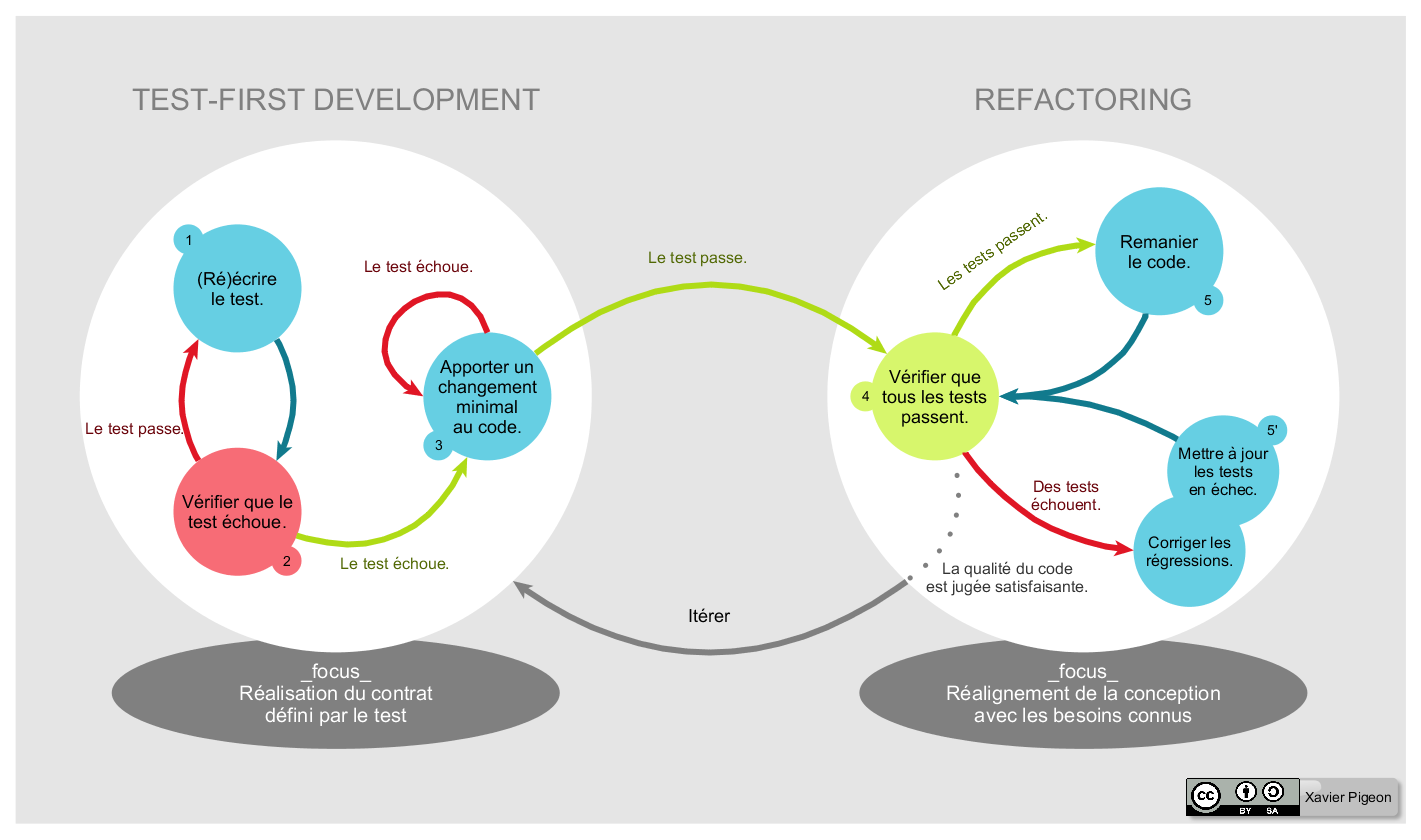
\includegraphics[width=0.5\textwidth]{fig/Cycle-global-tdd.png}
	\caption{Cycle Globale du Test Driven Développement  }
	\label{fig:TDD}
\end{figure}  
\begin{enumerate}
	\item écrire un premier test ;
	\item vérifier qu'il échoue (car le code qu'il teste n'existe pas), afin de vérifier que le test est valide ;
	\item écrire juste le code suffisant pour passer le test ;
	\item vérifier que le test passe ;
	\item puis réusiner le code, c'est-à-dire l'améliorer tout en gardant les mêmes fonctionnalités.
\end{enumerate}
\subsubsection{Avantages }
Ces tests permettent aussi de préciser les spécifications du code, et donc son comportement ultérieur en fonction des situations auxquelles il sera exposé. Ce qui facilite la production d'un code valide en toutes circonstances. On obtient donc un code plus juste et plus fiable. En écrivant les tests d'abord, on utilise le programme avant même qu'il existe. On s'assure ainsi que le code produit est testable unitairement. Il est donc impératif d'avoir une vision précise de la manière dont on va utiliser le programme avant même d'envisager son implémentation. Cela évite souvent des erreurs de conception dues à une précipitation dans l'implémentation avant d'avoir défini les objectifs.
\subsection{Fonctionnement de L'\ac{API}} 
Notre \ac{API} fonctionne selon le diagramme suivant :
\begin{figure}[H]
	\centering
	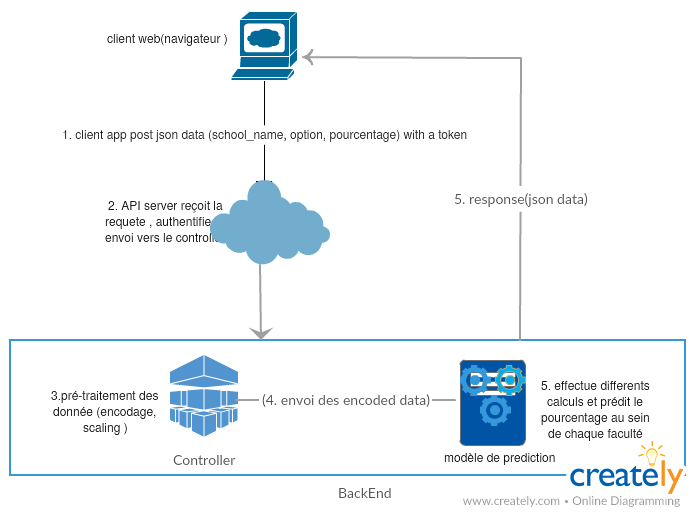
\includegraphics[width=0.5\textwidth]{fig/New-Predictive-Model.png}
	\caption{Flow chart de L'API }
	\label{fig:flowChart}
\end{figure}  
\begin{enumerate}
	\item le client we(navigateur ) envoi une requête post avec les données au format \ac{JSON} (non de l'école , l'option et le pourcentage du diplôme) et un token d'authentification 
	\item la requête est traité et authentifier et ensuite envoyer vers le contrôleur .
	\item  pré-traitement des données : les données sont encodés et échelonner 
	\item  prédiction : les calculs sont effectué par nos modèles de prédiction 
	\item le contrôleur renvoie différentes prédictions sous forme d'objet \ac{JSON} et sont affiché au navigateur.  
\end{enumerate}
Notons que l'API fonctionne selon le modèle \ac{MVC} simplifié (sans base des données).
\section{Conclusion Partielle }
Au chapitre précédent nous avons pu remarquer qu'il existait une forte corrélation entre le CGPA et l'option suivie par l'étudiant à l'école secondaire ,et entre l'école de provenance et le CGPA , mais nous avons aussi souligné qu'il n'existait pas de corrélation entre le CGPA et Le DIPERC mais nous avons décider de l'utiliser dans la prédiction du CGPA pour améliorer l'exactitude ne notre modèle et le rendre plus subjectif  .

Lors de l'entrainement de nos modèles nous avons pu remarquer qu'au sein de chaque faculté les modèles de régression linaire régularisée(Lasso,Elastic-Net et Ridge) disposent des meilleurs résultats avec une moyenne de \ac{RMSE}inférieur à 12\% tandis que les modèles SVM disposaient des résultats légèrement supérieur .
Ces Erreurs élevées étaient dues au fait :

\begin{itemize}
	\item Nous n'avons pas pu disposer de plusieurs variables du même type que le DIPPERC  c'est pourquoi pour réduire cet erreur nous devrions obtenir diverses variable du même type que le CGPA entre autre les valeurs des pourcentages obtenus à l'école secondaire car notre modèle a tendance à avantager le diplôme pourcentage en lui donnant un grand coefficient (0.67) en faculté de technologie et 0.47 en faculté de médecine. 
	\item Que nous ne disposions pas d'assez des données(exemples) pour entrainer nos algorithmes notre grand ensemble d'apprentissage disposaient de 900 éléments (moins de 1000 ) ce qui reste relativement  moins élevé   .
\end{itemize}

Pour palier a ces problème et dans le souci de réduire notre \ac{RMSE} nous avons utiliser la technique de stacking qui consistait à combiner les différentes résultats des différents modèles et à partir de ceux -ci prédire un résultat finale à l'aide d'une régression linéaire, nous avons souligné que cette technique réduisait l'erreur de prédiction considérablement et nous avons ainsi une erreur inférieure à 10\% dans certaines faculté.

